\documentclass[aspectratio=169]{beamer}
\usepackage[UTF8]{ctex}
\usepackage{graphicx}
\usepackage{booktabs}
\usepackage{hyperref}
\usepackage{tikz}
\usetikzlibrary{positioning,arrows.meta}
\usepackage{PekingU}

\title{AI 模拟面试官}
\subtitle{把一份简历，变成一场真实技术面试}
\author{16 小时 AI Agent 产品挑战}
\date{2026-05-10}
\logo{
\includegraphics[height=0.75cm]{pic/PKU_logo.png}}

\definecolor{pitchred}{RGB}{139,0,18}
\definecolor{pitchblue}{RGB}{36,95,170}
\definecolor{pitchcyan}{RGB}{40,170,185}
\definecolor{pitchgray}{RGB}{70,76,86}
\definecolor{pitchlight}{RGB}{245,248,250}
\setbeamerfont{frametitle}{size=\Large}

\newcommand{\bigclaim}[1]{%
  {\LARGE\bfseries #1}
}
\newcommand{\metric}[2]{%
  \begin{minipage}{0.18\linewidth}
    \centering
    {\Huge\bfseries\color{pitchred} #1}\\[-0.1em]
    {\small #2}
  \end{minipage}
}
\newcommand{\card}[2]{%
  \begin{beamercolorbox}[wd=\linewidth,rounded=true,sep=0.8em]{block body}
    \textbf{#1}\\[-0.15em]
    {\small #2}
  \end{beamercolorbox}
}
\newcommand{\screenshotbox}[2]{%
  \begin{center}
    \IfFileExists{#1}{\includegraphics[width=0.9\linewidth,height=0.50\textheight,keepaspectratio]{#1}}{\fbox{\begin{minipage}[c][0.46\textheight][c]{0.86\linewidth}\centering\Large #2\\[0.5em]\normalsize 截图占位\end{minipage}}}
  \end{center}
}

\begin{document}

\begin{frame}
  \titlepage
  \vspace{-0.4em}
  \centering
  \small 公网 Demo：\href{http://8.139.254.60:3000/}{http://8.139.254.60:3000/}
\end{frame}

\begin{frame}{一个高频但低质量的准备场景}
  \bigclaim{学生不缺资料，缺一位会追问自己简历的面试官。}
  \vspace{1.0em}
  \begin{columns}[T]
    \begin{column}{0.46\linewidth}
      \card{真实面试怎么问}{从简历项目切入，追个人贡献、技术取舍、坏例归因、指标验证和迁移能力。}
      \vspace{0.7em}
      \card{学生怎么准备}{刷题、背八股、改简历，但缺少高频、低成本、贴近个人项目的压力训练。}
    \end{column}
    \begin{column}{0.48\linewidth}
      \card{现有工具缺口}{ChatGPT 容易变知识讲解；题库无法结合个人简历；简历工具只能润色，不能模拟追问。}
      \vspace{0.7em}
      \card{我们的判断}{MVP 要做深做窄：上传简历，被连续追问，最后知道自己哪里会挂。}
    \end{column}
  \end{columns}
\end{frame}

\begin{frame}{用户洞察来自 456 条结构化输入}
  \centering
  \metric{456}{调研输入}\hfill
  \metric{158}{小红书面经}\hfill
  \metric{204}{追问链样本}\hfill
  \metric{50}{岗位 JD}\hfill
  \metric{8}{竞品体验}
  \vspace{1.1em}

  \begin{tikzpicture}[x=0.55cm,y=0.45cm]
    \node[anchor=east] at (0,0) {项目深挖};\fill[pitchblue] (0.25,-0.16) rectangle (8.8,0.16);\node[anchor=west] at (9.0,0) {114};
    \node[anchor=east] at (0,-0.75) {八股基础};\fill[pitchblue] (0.25,-0.91) rectangle (7.4,-0.59);\node[anchor=west] at (7.6,-0.75) {95};
    \node[anchor=east] at (0,-1.50) {算法/手撕};\fill[pitchblue] (0.25,-1.66) rectangle (7.2,-1.34);\node[anchor=west] at (7.4,-1.50) {92};
    \node[anchor=east] at (0,-2.25) {LLM 专项};\fill[pitchcyan] (0.25,-2.41) rectangle (5.3,-2.09);\node[anchor=west] at (5.5,-2.25) {67};
    \node[anchor=east] at (0,-3.00) {追问压力};\fill[pitchcyan] (0.25,-3.16) rectangle (5.3,-2.84);\node[anchor=west] at (5.5,-3.00) {67};
    \node[anchor=east] at (0,-3.75) {焦虑/不确定};\fill[pitchgray] (0.25,-3.91) rectangle (3.9,-3.59);\node[anchor=west] at (4.1,-3.75) {48};
  \end{tikzpicture}
  \vspace{0.4em}

  \small 最高频信号不是“缺题”，而是项目深挖、八股落地、手撕代码和 LLM/Agent 专项都需要和简历结合。
\end{frame}

\begin{frame}{产品解法：一场围绕简历展开的训练闭环}
  \begin{center}
    \begin{tikzpicture}[node distance=0.55cm, every node/.style={font=\small}]
      \node[draw,rounded corners,fill=pitchlight,minimum width=2.5cm,minimum height=0.9cm] (a) {上传 PDF 简历};
      \node[draw,rounded corners,fill=pitchlight,right=0.9cm of a,minimum width=2.5cm,minimum height=0.9cm] (b) {AI 连续追问};
      \node[draw,rounded corners,fill=pitchlight,right=0.9cm of b,minimum width=2.5cm,minimum height=0.9cm] (c) {暴露挂点};
      \node[draw,rounded corners,fill=pitchlight,right=0.9cm of c,minimum width=2.5cm,minimum height=0.9cm] (d) {结构化复盘};
      \draw[-{Latex[length=2.5mm]},thick,pitchblue] (a) -- (b);
      \draw[-{Latex[length=2.5mm]},thick,pitchblue] (b) -- (c);
      \draw[-{Latex[length=2.5mm]},thick,pitchblue] (c) -- (d);
      \draw[-{Latex[length=2.5mm]},dashed,pitchcyan] (d.south) .. controls +(down:1.0cm) and +(down:1.0cm) .. (a.south);
    \end{tikzpicture}
  \end{center}
  \vspace{0.8em}
  \begin{columns}[T]
    \begin{column}{0.48\linewidth}
      \card{专项强化}{八股知识点、简历经历、手撕代码，分别训练知识、项目和 coding。}
    \end{column}
    \begin{column}{0.48\linewidth}
      \card{完整模拟}{AI 根据简历和前序回答决定下一问，覆盖项目、相关八股、手撕和综合追问。}
    \end{column}
  \end{columns}
\end{frame}

\begin{frame}{Demo Wow Moment：PDF 简历一键进入完整模拟}
  \screenshotbox{screenshots/pdf-resume-loaded.png}{PDF 样例简历已加载}
  \small
  这份样例简历由 LaTeX 生成，包含 RAG、Agent、Redis 和后端工程经历。系统解析文本层 PDF 后，完整模拟会围绕这些真实风险点追问。
\end{frame}

\begin{frame}{产品界面：四个入口，不是一锅聊天}
  \screenshotbox{screenshots/home.png}{四入口训练工作台}
  \small
  首页先让用户选择训练目标，避免八股、简历深挖和手撕代码互相污染；每个训练入口维护独立会话。
\end{frame}

\begin{frame}{核心引擎：Agentic RAG 面试官}
  \begin{center}
    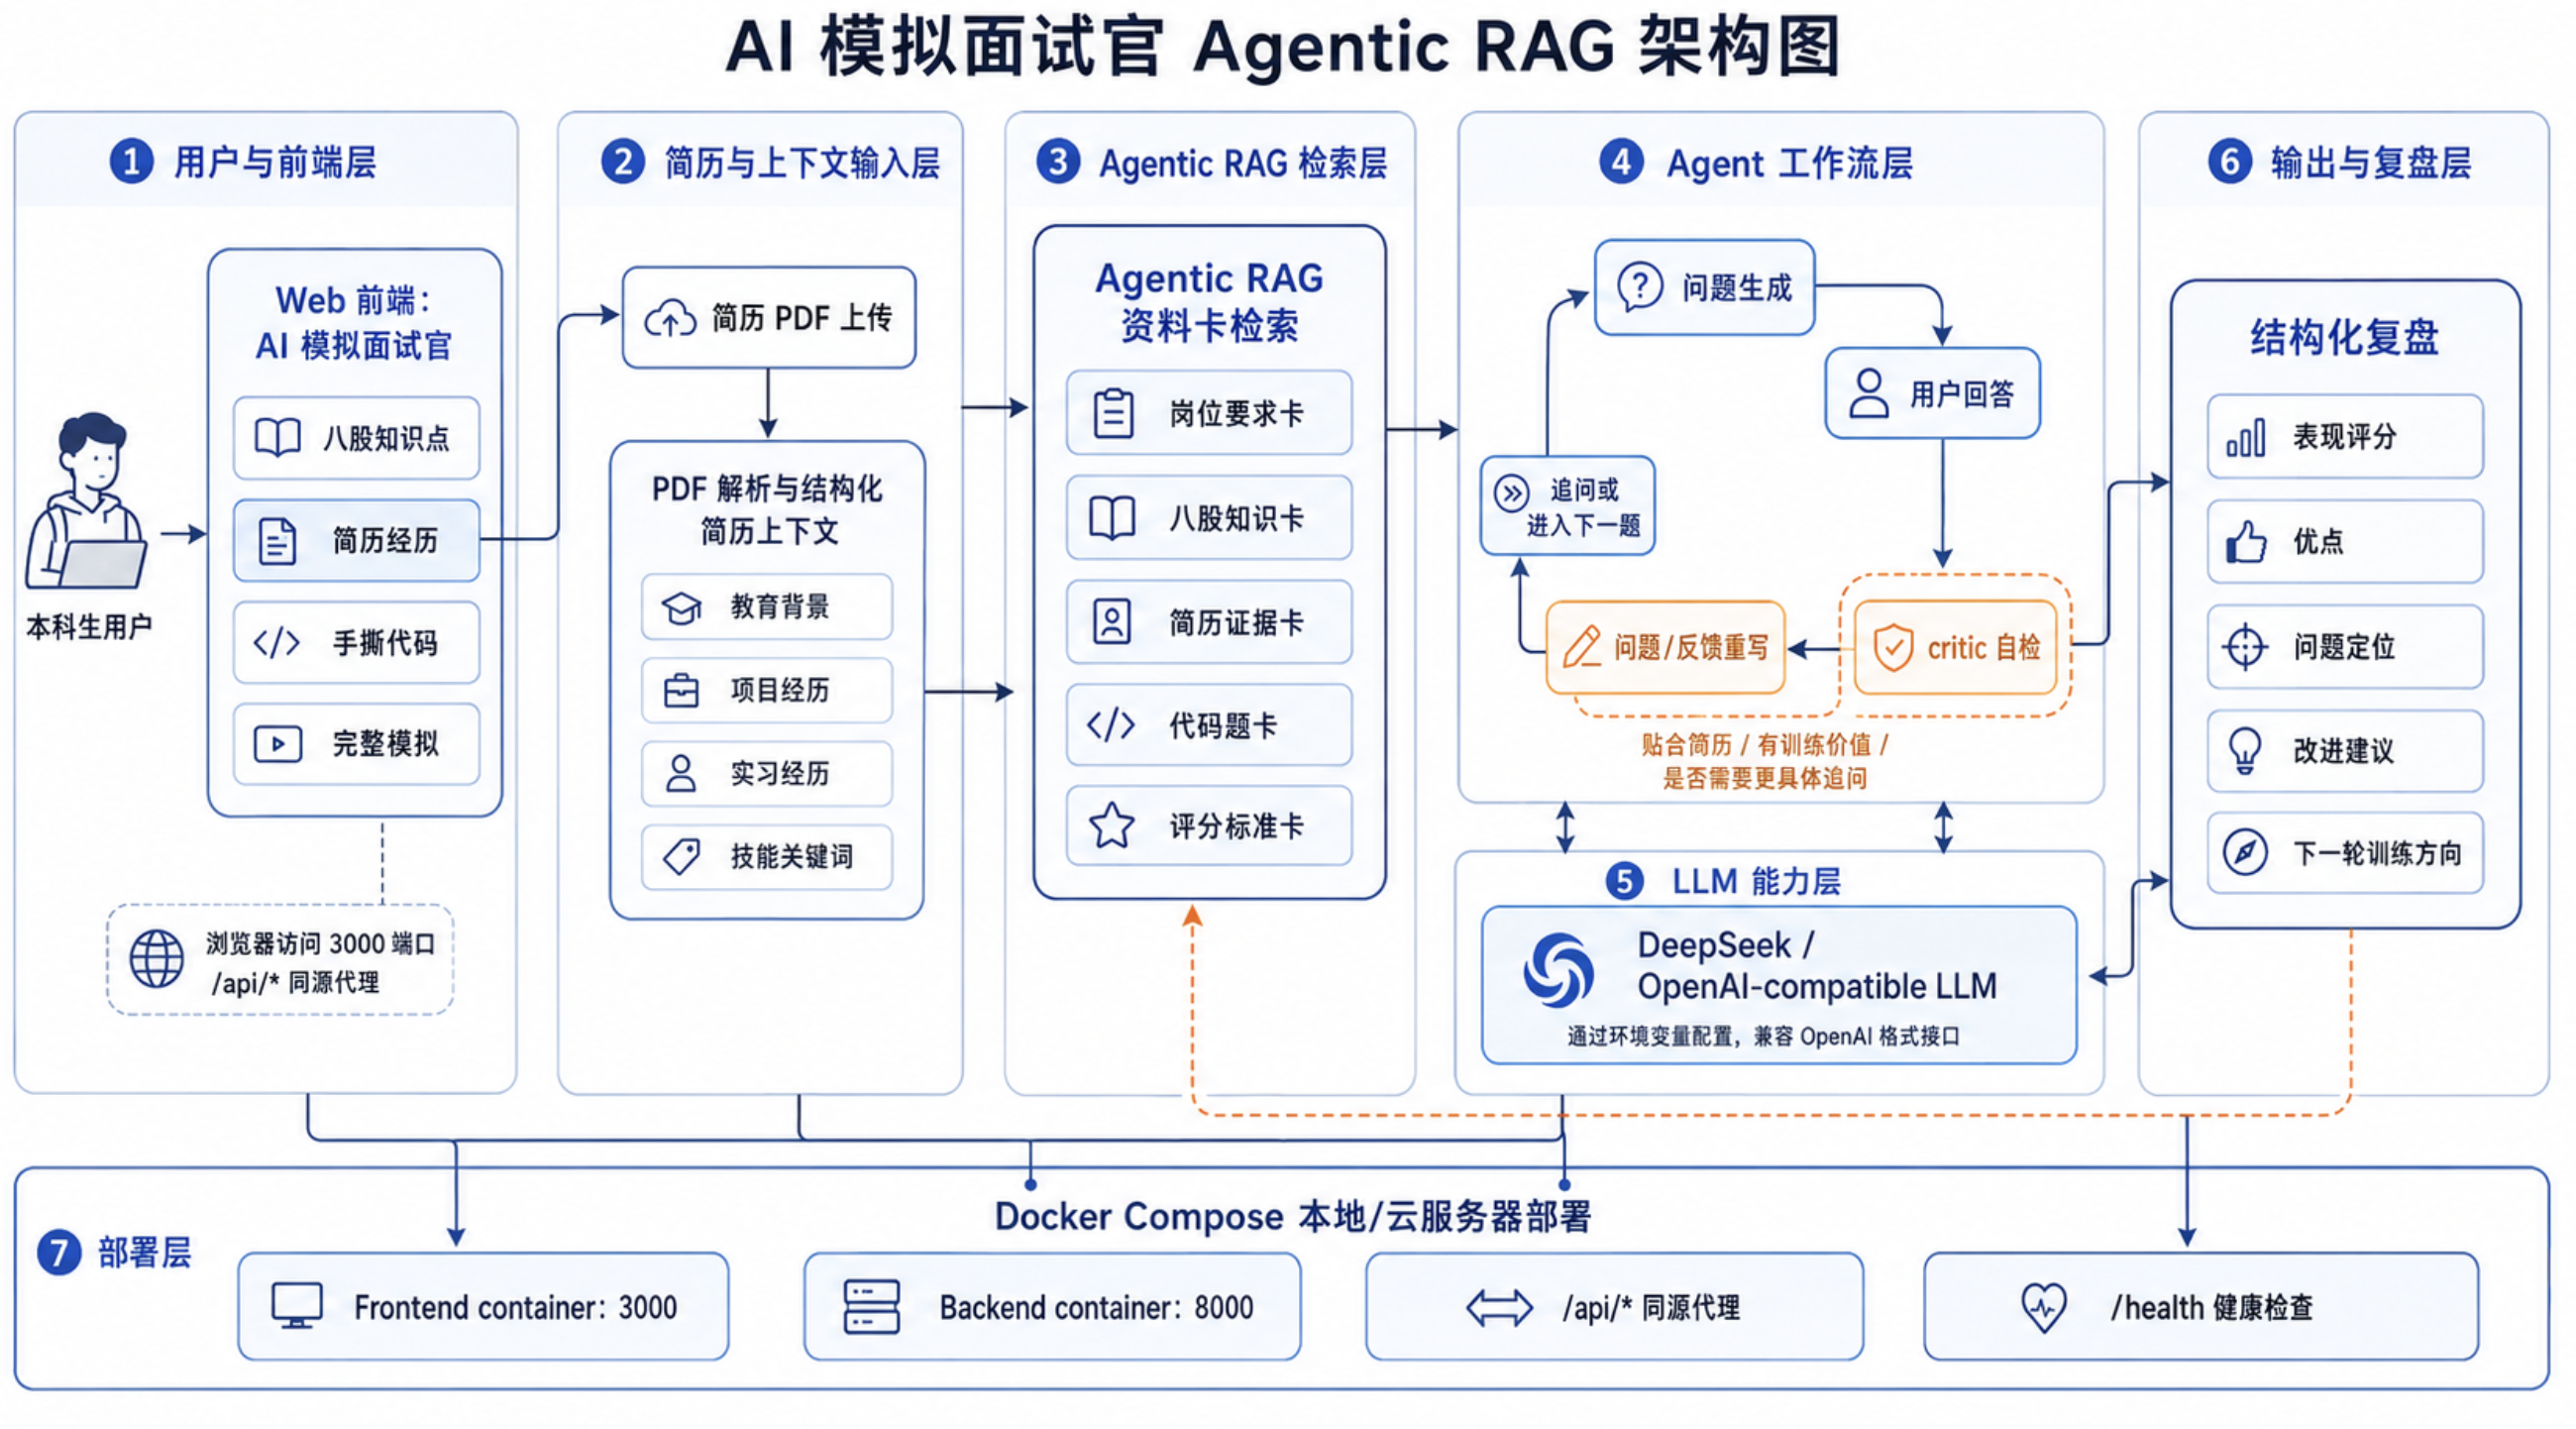
\includegraphics[width=\linewidth,height=0.72\textheight,keepaspectratio]{fig/image.png}
  \end{center}
  \small
  不是简单 RAG 问答：系统把简历解析、资料卡检索、问题生成、critic 自检、LLM 能力和结构化复盘串成一个训练闭环。
\end{frame}

\begin{frame}{差异化：从“会回答问题”到“会训练用户”}
  \begin{table}
    \small
    \begin{tabular}{p{0.22\linewidth}p{0.31\linewidth}p{0.34\linewidth}}
      \toprule
      维度 & 普通聊天机器人 & AI 模拟面试官 \\
      \midrule
      输入 & 用户自己描述问题 & 简历 PDF + 目标岗位 + 历史回答 \\
      互动 & 回答用户提问 & 主动发现漏洞并追问 \\
      依据 & 上下文引用不稳定 & 展示简历证据、风险假设、资料卡 \\
      复盘 & 泛泛建议 & 挂点、评分维度、下一轮行动 \\
      \bottomrule
    \end{tabular}
  \end{table}
  \vspace{0.4em}
  \centering
  \large\textbf{产品价值不是“问更多题”，而是让用户更快发现真实面试里的失败点。}
\end{frame}

\begin{frame}{商业目标：先验证训练价值，再做增长}
  \begin{columns}[T]
    \begin{column}{0.48\linewidth}
      \card{MVP KPI}{简历上传激活率、3 轮训练完成率、复盘生成率、24 小时复练率、复盘有用性评分。}
      \vspace{0.7em}
      \card{成本结构}{主要成本是 LLM token、云服务器和文件解析；文字训练比语音/视频更利于早期控成本。}
    \end{column}
    \begin{column}{0.48\linewidth}
      \card{商业路径}{Freemium：免费限次训练，付费解锁完整模拟、历史报告、JD 匹配和复练计划。}
      \vspace{0.7em}
      \card{B 端机会}{高校就业中心、求职社团、训练营和实验室可购买批量账号与训练数据看板。}
    \end{column}
  \end{columns}
\end{frame}

\begin{frame}{未来路线图}
  \begin{center}
    \begin{tabular}{p{0.22\linewidth}p{0.22\linewidth}p{0.22\linewidth}p{0.22\linewidth}}
      \toprule
      \textbf{1 周} & \textbf{2--3 周} & \textbf{1 个月} & \textbf{2--3 个月} \\
      \midrule
      JD 匹配 & 复练体系 & 语音压力面 & 高校试点 \\
      历史训练记录 & 资料库扩充 & 趋势报告 & 付费转化 \\
      \bottomrule
    \end{tabular}
  \end{center}
  \vspace{1em}
  \small 下一步资源需求：产品/增长负责访谈和指标，全栈负责账号与历史记录，LLM 工程负责资料卡、评测集和 rubric。
\end{frame}

\begin{frame}{今天交付}
  \begin{itemize}
    \item 产品链接：\href{http://8.139.254.60:3000/}{http://8.139.254.60:3000/}
    \item GitHub：\href{https://github.com/JianzheLi/aiic-project}{https://github.com/JianzheLi/aiic-project}
    \item 技术栈：FastAPI + Vite/React + Docker Compose，浏览器只访问 3000。
    \item 提交材料：Demo 视频、Product Memo、Beamer 路演 PPT、LaTeX 假简历、调研报告。
    \item 服务器：已按挑战要求追加 2 个评审 SSH 公钥。
  \end{itemize}
\end{frame}

\end{document}
